%necessary tikz libraries
%\usetikzlibrary{tikzmark,arrows,positioning}
\begin{figure}
  \centering
  \begin{minipage}[c]{.5\textwidth}
    \centering
    \begin{cxt}%
      \cxtName{}%
     \att{\tikzmarknode{ca1}{1}}%
     \att{\tikzmarknode{ca4}{4}}%
     \att{\tikzmarknode{ca3}{3}}%
     \att{\tikzmarknode{ca2}{2}}%
     \att{\tikzmarknode{ca5}{5}}%
      \obj{x.x..}{1}
      \obj{x.x..}{4}
      \obj{.x.x.}{2}
      \obj{....x}{3}
    \end{cxt}
  \end{minipage}%
  \begin{minipage}[c]{.5\textwidth}
    \centering
    \colorlet{mivertexcolor}{blue}
    \colorlet{jivertexcolor}{red}
    \colorlet{vertexcolor}{mivertexcolor!50}
    \colorlet{bordercolor}{black!80}
    \colorlet{linecolor}{gray}
    \tikzset{vertexbase/.style={semithick, shape=circle, inner sep=2pt, outer sep=0pt, draw=bordercolor},%
      vertex/.style={vertexbase, fill=vertexcolor!45},%
      mivertex/.style={vertexbase, fill=mivertexcolor!45},%
      jivertex/.style={vertexbase, fill=jivertexcolor!45},%
      divertex/.style={vertexbase, top color=mivertexcolor!45, bottom color=jivertexcolor!45},%
      conn/.style={-, thick, color=linecolor}%
    }
    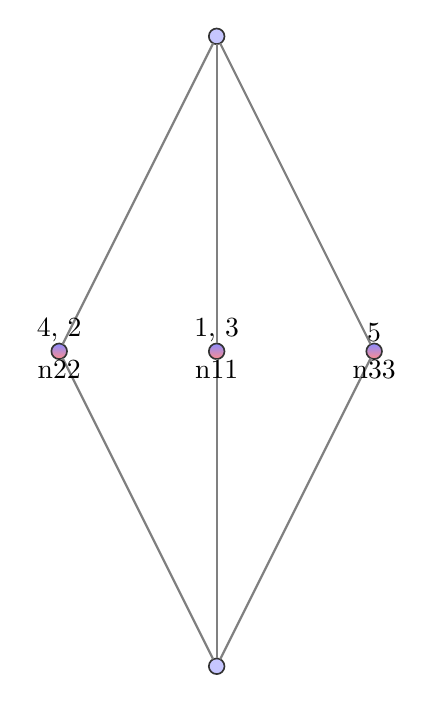
\begin{tikzpicture}
      \begin{scope} %for scaling and the like
        \begin{scope} %draw vertices
          \foreach \nodename/\nodetype/\xpos/\ypos in {%
        0/vertex/0/0,
        1/divertex/-2/4,
        2/divertex/0/4,
        3/divertex/2/4,
        4/vertex/0/8
          } \node[\nodetype] (\nodename) at (\xpos, \ypos) {};
        \end{scope}
        \begin{scope} %draw connections
    \path (1) edge[conn] (4);
    \path (0) edge[conn] (1);
    \path (0) edge[conn] (2);
    \path (0) edge[conn] (3);
    \path (2) edge[conn] (4);
    \path (3) edge[conn] (4);
        \end{scope}
        \begin{scope} %add labels
          \foreach \nodename/\labelpos/\labelopts/\labelcontent in {%
            1/below//{\tikzmarknode{n2}{}2},
            1/above//{4, 2},
            2/below//{\tikzmarknode{n1}{}1},
            2/above//{1, 3},
            3/below//{\tikzmarknode{n3}{}3},
            3/above//{5}
          } \coordinate[label={[\labelopts]\labelpos:{\labelcontent}}](c) at (\nodename);
        \end{scope}
      \end{scope}
    \end{tikzpicture}
  \end{minipage}%
\end{figure}
\begin{tikzpicture}[overlay,remember picture]
  \node[right = 0.45cm of ca2] (za) {};
  \node[below = 0.25cm of za] (co1) {};
  \node[below = 0.16cm of co1] (co4) {};
  \node[below = 0.16cm of co4] (co2) {};
  \node[below = 0.16cm of co2] (co3) {};
  \node[above = 0.2cm of n1] (an1) {};
  \node[above = 0.2cm of n3] (an3) {};
  \node[above = 0.2cm of n2] (an2) {};
  \draw[->, >=stealth] (co1) -- (an1);
  \draw[->, >=stealth] (co4) -- (an1);
  \draw[->, >=stealth] (co2) -- (an1);
  \draw[->, >=stealth] (co3) -- (an2);
\end{tikzpicture}
